\documentclass[a4paper, 12 pt]{article}
\usepackage[utf8]{inputenc}
\usepackage[T1]{fontenc}
\usepackage[slovene]{babel}
\usepackage{lmodern}
\usepackage{mathrsfs}
\usepackage{subfig}
\usepackage[pdftex]{graphicx}
\usepackage{float}


%\graphicspath{{.\wiener-inverse-interval-problem\slike\Porocilo}}



\pagenumbering{arabic}


\begin{document}

\begin{titlepage}

\begin{center}



\Huge
\textbf{Skupina 6: Wiener inverse interval problem}

\vspace{0.5cm}
\large{Projekt v povezavi s predmetom Operacijske raziskave}

\vspace{2.5cm}
\Large
\textbf{Končno poročilo}

\vspace{2.5cm}
\large
Avtorja: \\
\textbf{Tjaša Renko, Darjan Pavšič}

\vfill

\large{Ljubljana, november 2019}


\end{center}
\end{titlepage}


\tableofcontents

\vspace{1cm}

\listoffigures

\pagebreak

\section{Predstavitev problema}

\subsection{Problem P1}

Za fiksno število vozlišč $n$ in drevo $T$ naj bo $\mathscr{T}_{n+1}$ množica vseh dreves na $n+1$ vozliščih, dobljena iz $T$ z dodajanjem lista enemu iz vozlišč $T$. $W(\mathscr{T}_{n+1})$ pa množica vrednosti Wienerjevega indeksa za drevesa iz $\mathscr{T}_{n+1}$. Poiskati želimo tako drevo $T$ na $n$ vozliščih, da bo moč množice $W(\mathscr{T}_{n+1})$ čim manjša (čim večja).


\subsection{Problem P2}

Za fiksno število vozlišč $n$ iščemo drevo $T$ z največjim možnim premerom, da bo veljalo; obstajata list $u$, pripet na vozlišče $v$, in vozlišče $w$ iz $T$, da je list $u$ tak, da z odstranitvijo povezave $uv$ in dodajanjem $uw$ spremenimo vrednost indeksa za 1.

\subsection{Izbira programskega jezika in knjižnic}

Za izvedbo naloge sva se odločila za programski jezik \textit{Python}, za lažje delo z grafi pa sva si pomagala s knjižnico \texttt{networkx}, tako da sva grafe lahko predstavljala kot objekte, sposodila pa sva si tudi vgrajeni funkciji računanja poti med poljubnima vozliščema grafa ter računanja premera. Uporabljala sva tudi knjižnice \texttt{numpy}, \texttt{random} in pa \texttt{matplotlib}, s katero so grafi tudi vizualno predstavljeni.



\pagebreak

\section{Problem P1}

\subsection{Reševanje}

Zaradi velike časovne zahtevnosti sva problem ločila na eno kodo, ki išče točno rešitev in je uporabna za grafe z majhnim številom vozlišč, ter drugo, časovno in prostorsko bolj optimalno, ki si prizadeva najti dober približek točne rešitve za večje grafe.
\vspace{0.5cm}

Glavni del kode za iskanje točnih rešitev se nahaja v datoteki z imenom \textit{p1\_manjsi\_grafi.py}. Tam so definirane funkcije za iskanje Wienerjevega indeksa s pomočjo najkrajših poti med posameznima točkama drevesa, generiranje množice $\mathscr{T}_{n+1}$  z računanjem indeksov glede na indeks prvotnega drevesa ter iskanje optimumov. \\

Rešitev iščemo tako, da poženemo \textit{shranjevanje\_manjsi\_grafi\_p1.py} ter v funkciji \textit{zapisi\_resitve} nastavimo za argument željeno število vozlišč drevesa, do katerega želimo imeti rezultate. Za število vozlišč $n$ ne priporočava izbire števila, večjega od 17. Pri $n$ = 20 že dobimo opozorilo \textit{"memory error"}, ki bi se sicer dal odpraviti, a to nima smisla, saj nam bo prilagojen algoritem za tako majhne grafe ob pravilni izbiri parametrov zelo verjetno dal točno rešitev mnogo hitreje.
\vspace{0.5cm}

\begin{figure}[H]
    \centering
    \subfloat[Sodo število vozlišč, $n$ = 12]{{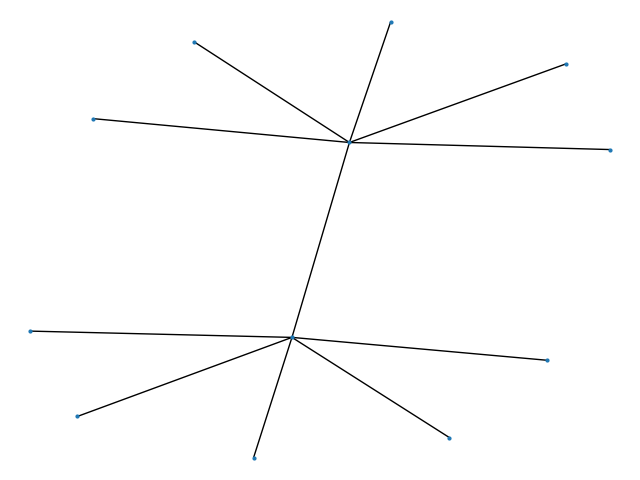
\includegraphics[width=6cm]{drevo12min2.png} }}
    \qquad
    \subfloat[Liho število vozlišč, $n$ = 13]{{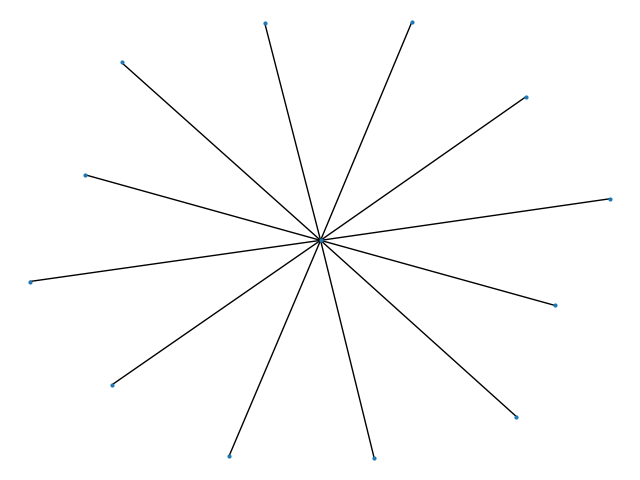
\includegraphics[width=6cm]{drevo13min2.png} }}
    \caption{Rešitvi za minimum, dobljeni s kodo za točne rešitve.}
    \label{p1min}
\end{figure}

\pagebreak

Glavni del kode za iskanje približkov na velikih grafih pa se nahaja v datoteki z imenom \textit{p1\_vecji\_grafi.py}, koda se požene iz datoteke \textit{shranjevanje\_vecji\_grafi\_p1.py}, tako da v funkciji \textit{shrani\_resitve} za argumente nastavimo seznam s števili, ki predstavljajo velikost grafov, za katere želimo rezultate; število korakov izvedbe \textit{simuliranega ohlajanja} za vsak graf; število dreves za odstranitev iz prvotnega seznama ter število dreves z istim številom vozlišč za prvotni seznam, iz katerega bomo naredili prej omenjeni ožji izbor za ohlajanje.\\

Za začetek reševanja tega problema sva potrebovala ustrezne grafe. Ker naključna drevesa navadno ne bodo dovolj dobra, sva generirala nekaj boljših s pomočjo modificiranega \textit{Kruskalovega algoritma} tako, da sva vzela pot velikosti nekje med 80 in 95\% števila vseh vozlišč in nato naključno dodajala povezave na pot tako, da je nastalo povezano drevo, kar se je izkazalo za zelo učinkovito.\\

Za časovno optimalno računanje Wienerjevih indeksov sva najprej shranila dolžine najkrajših poti med vsakima točkama grafa. Tako sva potem lahko izračunala indeks vsakega posameznega novega drevesa v linearnem času; potrebovala sva namreč le vsoto poti iz vozlišča, ki sva mu dodala list, vsoto vseh poti ter število vozlišč; vse te podatke pa sva že imela. \\

 Ko sva dobila podatke za na začetku generirana drevesa, sva med temi izbrala boljša in na njih izvedla algoritem za iskanje lokalnih ekstremov v okolici grafa, in sicer vrsto metahevristike z imenom \textit{simulirano ohlajanje}. Ta na vsakem koraku preveri stanje sosednjega grafa in se s padajočo verjetnostjo odloča, ali se bo vanj preselila, hkrati pa shranjuje najboljši rezultat do sedaj. \\

Sosednji graf za algoritem sva ustvarila tako, da sva od prejšnjega odstranila povezavo z naključnega lista in naredila naključno novo iz njega, vzela pa sva po uporabi zelo razširjeno \textit{Kirkpatrickovo funkcijo} za spreminjanje verjetnosti. Število korakov ohlajanja se prilagaja glede na število vozlišč. Po končanem algoritmu \textit{simuliranega ohlajanja} je bilo treba samo še poiskati najboljšega izmed vseh rezultatov.
\pagebreak

\begin{figure}[H]
\centering
  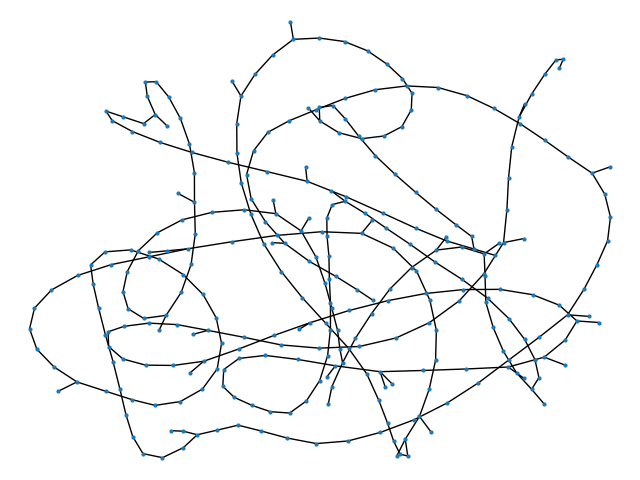
\includegraphics[width=9cm]{drevo300max295.png}
  \caption{Primer dobljenega grafa za maksimum preko simuliranega ohlajanja}
  \label{fig:300max} 
\end{figure}

\subsection{Časovna zahtevnost}

Časovno zahtevnost kode s simuliranim ohlajanjem sva preverila tudi eksperimentalno za nekaj različnih vrednosti števila vozlišč $n$. Pri parametrih: št. grafov = 1, število korakov ohjanja ($kmax$) = 20, število dreves za odstanitev = 48, število dreves za izbiro = 50 sva dobila sledeče rezultate: \\

\begin{figure}[H]
\centering
  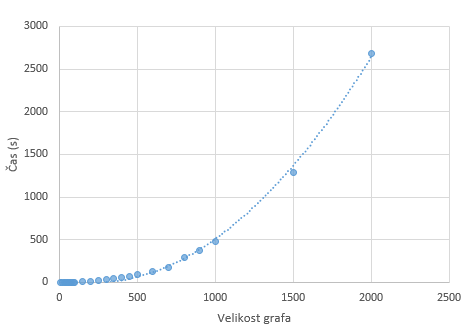
\includegraphics[width=9cm]{casovna_p1_n.png}
  \caption{Časovna zahtevnost glede na različno število vozlišč}
  \label{fig:p1_časovna_zaht_n} 
\end{figure}

\pagebreak
Pri fiksnem številu vozlišč na $n$ = 100 pa je časovna zahtevnost glede na število korakov ohlajanja linearna:

\begin{figure}[H]
\centering
  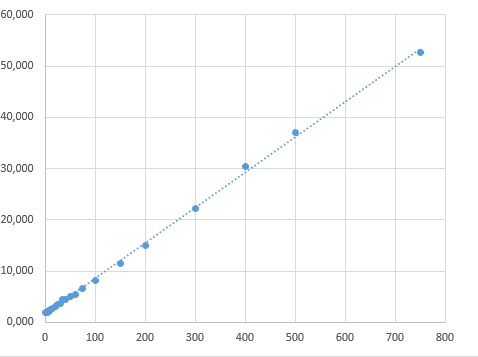
\includegraphics[width=9cm]{casovna_p1_kmax.png}
  \caption{Časovna zahtevnost glede na število korakov ohlajanja}
  \label{fig:p1_časovna_zaht_kmax} 
\end{figure}

Časovna zahtevnost se ob spreminjanju \textit{začetne temperature} pri simuliranem ohlajanju ni kaj dosti spreminjala tako pri grafih z $n$ = 100 kot pri grafih z $n$ = 1000 vozlišči, torej kot kaže ta parameter na le-to nima bistvenega vpliva, seveda pa mora biti vrednost večja od 0.

\subsection{Rezultati in povzetek}

Meniva, da sva našla globalni minimum za poljubno število vozlišč, da je enak $2$ in je dosežen pri zvezdah. Našla pa sva še en minimum za soda števila vozlišč $n$, sestavljen iz dveh zvezd velikosti $n/2$, povezanih s središčema. Kar se tiče maksimumov, jih je, sodeč po točnih rešitvah na manjših grafih in uspešnostjo algoritmov na večjih, precej veliko in so običajno po velikosti malo pod številom vozlišč ter največ enaki. Njihovo obliko si lahko ogledamo v mapi s shranjenimi slikami, vidimo pa, da imajo precej velik premer.

\pagebreak

\section{Problem P2}

\subsection{Reševanje}

Za manjše grafe, kjer je možno eksaktno računanje, sva napisala funkcijo za generiranje vseh izomorfnih dreves na $n$ vozliščih ter funkcije, ki najprej iz vseh poberejo tista z iskano lastnostjo, to je spremembo Wienerjevega indeksa za 1 ob odstranitvi ene in dodajanju nove povezave kot v opisu problema, nato pa izmed teh vrnejo tisto drevo z največjim premerom, če tako sploh obstaja. To je točna rešitev problema, a je časovno zahtevna ne le generacija grafov, temveč tudi računanje premera. Zato sva za večje $n$ tudi tukaj napisala novo kodo. \\

\begin{figure}[H]
\centering
  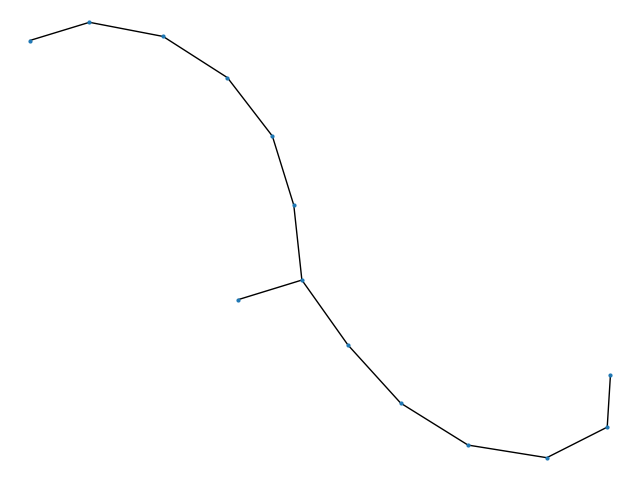
\includegraphics[width=7cm]{drevo14diam12.png}
  \caption{Primer točne rešitve za število vozlišč $n$ = 14, premer = 12}
  \label{fig:graf1}
\end{figure}

Ideja algoritma za iskanje drevesa na večjem številu vozlišč pri P2 je, da začneva na poti z željenim številom vozlišč in za njo posebej izračunava wienerjev indeks na časovno preprost način. Nato na vsakem koraku odstraniva povezavo iz lista in dodava novo ter glede na prejšnji graf izračunava nov indeks ter ju primerjava, nato pa star graf nadomestiva z novim. To omogoča preverjanje velikega števila grafov, kar je za problem P2 ključno.\\

\begin{figure}[H]
\centering
  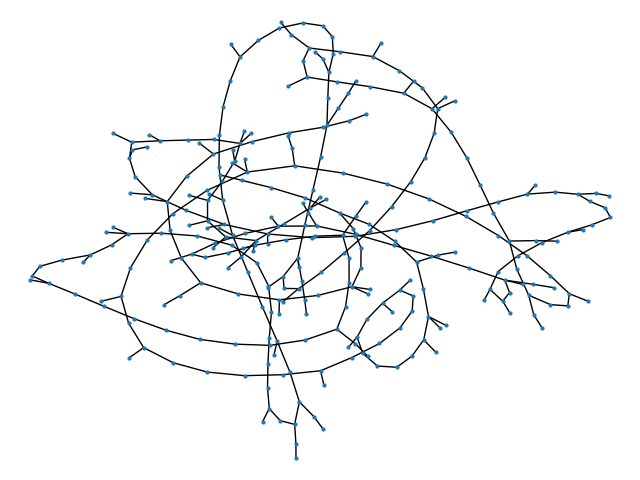
\includegraphics[width=12cm]{drevo300diam202.png}
  \caption{Primer dobljenega grafa na $n$ = 300 vozliščih s kodo za večje grafe}
  \label{300_p2} 
\end{figure}

\subsection{Časovna zahtevnost}

Tudi tukaj sva eksperimentalno preverila časovno zahtevnost kode pri različnih vrednostih spremenljivk. Pri spreminjajočem številu vozlišč $n$ je ob $1 \ 000 \ 000$ korakih algoritma sledeča:

\begin{figure}[H]
\centering
  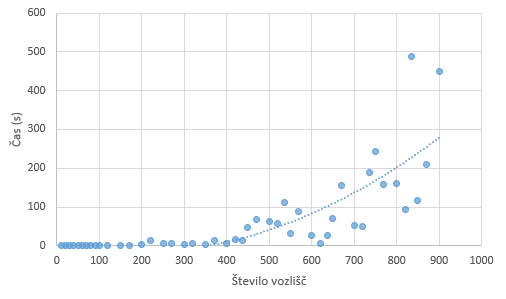
\includegraphics[width=9cm]{casovna_p2_n.png}
  \caption{Časovna zahtevnost glede na število vozlišč}
  \label{fig:p2_časovna_zaht_n} 
\end{figure}

\pagebreak

Še časovna zahtevnost pri fiksnem številu vozlišč $n = 200$ in $n$ = 6000 ter različnem številu korakov algoritma (koraki so izraženi v tisoč):

\begin{figure}[H]
    \centering
    \subfloat[Število vozlišč $n$ = 200, program najde ustrezno drevo]{{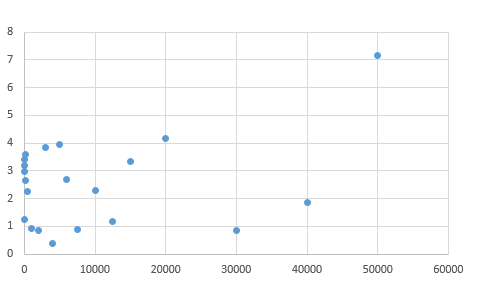
\includegraphics[width=6cm]{casovna_p2_korak.png} }}
    \qquad
    \subfloat[Število vozlišč $n$ = 6000, program ne najde ustreznega drevesa]{{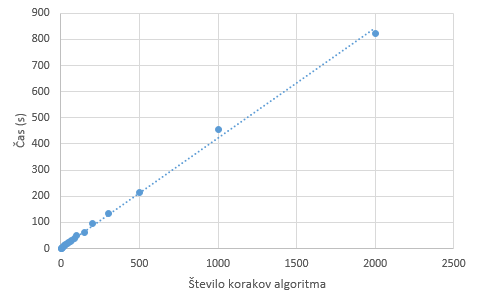
\includegraphics[width=6cm]{casovna_p2_korak_6000vozl.png} }}
    \caption{Časovna zahtevnost glede na število korakov algoritma}
    \label{p2korak}
\end{figure}


\subsection{Rezultati in povzetek}

Očitno je dobrih dreves precej malo, vsekakor dosti manj kot pri P1, saj je treba izvesti ogromno število korakov spreminjanja, da najdemo vsaj eno; to pa še narašča s številom vozlišč; pri $n$ = 2000 namreč morda celo $1 \ 000 \ 000$ korakov ni dovolj. Videti je, da najin algoritem dobiva maksimume v velikosti okoli treh četrtin števila vozlišč. Težko je oceniti kvaliteto rešitev s pomočjo točnih rešitev manjših grafov, saj je ta koda tako časovno zahtevna, da imava točne rezultate le do dreves s številom vozlišč $n$ = 14. Opazila sva tudi, da ne moreva dobiti iskanega drevesa za liho število vozlišč, in to ne le s poskušanjem, ampak tudi na malih grafih. Predpostavljava, da ne obstaja.

\end{document}
